\section{mo\-Tabu\-List$<$ M $>$ Class Template Reference}
\label{classmo_tabu_list}\index{moTabuList@{moTabuList}}
Class describing a tabu list that a {\bf mo\-TS}{\rm (p.\,\pageref{classmo_t_s})} uses.  


{\tt \#include $<$mo\-Tabu\-List.h$>$}

Inheritance diagram for mo\-Tabu\-List$<$ M $>$::\begin{figure}[H]
\begin{center}
\leavevmode
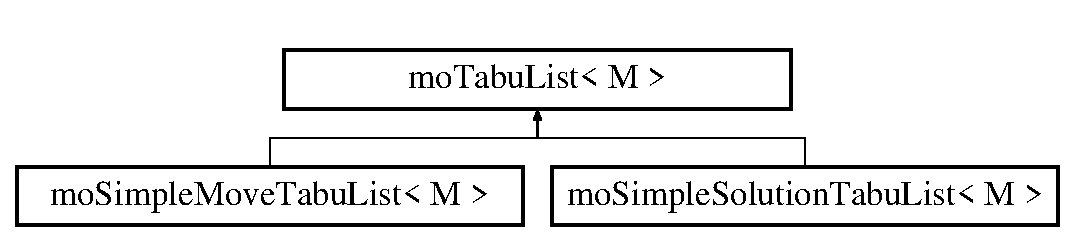
\includegraphics[height=3.88889cm]{classmo_tabu_list}
\end{center}
\end{figure}
\subsection*{Public Types}
\begin{CompactItemize}
\item 
typedef M::EOType {\bf EOT}\label{classmo_tabu_list_w0}

\begin{CompactList}\small\item\em Alias for the type. \item\end{CompactList}\end{CompactItemize}
\subsection*{Public Member Functions}
\begin{CompactItemize}
\item 
virtual void {\bf add} (const M \&\_\-move, const {\bf EOT} \&\_\-solution)=0
\begin{CompactList}\small\item\em Procedure to add a move in the tabu list. \item\end{CompactList}\item 
virtual void {\bf update} ()=0
\begin{CompactList}\small\item\em Procedure that updates the tabu list content. \item\end{CompactList}\item 
virtual void {\bf init} ()=0
\begin{CompactList}\small\item\em Procedure which initialises the tabu list. \item\end{CompactList}\end{CompactItemize}


\subsection{Detailed Description}
\subsubsection*{template$<$class M$>$ class mo\-Tabu\-List$<$ M $>$}

Class describing a tabu list that a {\bf mo\-TS}{\rm (p.\,\pageref{classmo_t_s})} uses. 

It is only a description, does nothing... A new object that herits from this class has to be defined in order to be used in a {\bf mo\-TS}{\rm (p.\,\pageref{classmo_t_s})}. 



Definition at line 46 of file mo\-Tabu\-List.h.

\subsection{Member Function Documentation}
\index{moTabuList@{mo\-Tabu\-List}!add@{add}}
\index{add@{add}!moTabuList@{mo\-Tabu\-List}}
\subsubsection{\setlength{\rightskip}{0pt plus 5cm}template$<$class M$>$ virtual void {\bf mo\-Tabu\-List}$<$ M $>$::add (const M \& {\em \_\-move}, const {\bf EOT} \& {\em \_\-solution})\hspace{0.3cm}{\tt  [pure virtual]}}\label{classmo_tabu_list_a0}


Procedure to add a move in the tabu list. 

The two parameters have not to be modified so they are constant parameters.

\begin{Desc}
\item[Parameters:]
\begin{description}
\item[{\em \_\-move}]a new tabu move. \item[{\em \_\-solution}]the origianl solution associated to this move. \end{description}
\end{Desc}


Implemented in {\bf mo\-Simple\-Move\-Tabu\-List$<$ M $>$} {\rm (p.\,\pageref{classmo_simple_move_tabu_list_a2})}, and {\bf mo\-Simple\-Solution\-Tabu\-List$<$ M $>$} {\rm (p.\,\pageref{classmo_simple_solution_tabu_list_a2})}.\index{moTabuList@{mo\-Tabu\-List}!update@{update}}
\index{update@{update}!moTabuList@{mo\-Tabu\-List}}
\subsubsection{\setlength{\rightskip}{0pt plus 5cm}template$<$class M$>$ virtual void {\bf mo\-Tabu\-List}$<$ M $>$::update ()\hspace{0.3cm}{\tt  [pure virtual]}}\label{classmo_tabu_list_a1}


Procedure that updates the tabu list content. 

Generally, a counter associated to each saved move is decreased by one. 

Implemented in {\bf mo\-Simple\-Move\-Tabu\-List$<$ M $>$} {\rm (p.\,\pageref{classmo_simple_move_tabu_list_a3})}, and {\bf mo\-Simple\-Solution\-Tabu\-List$<$ M $>$} {\rm (p.\,\pageref{classmo_simple_solution_tabu_list_a3})}.\index{moTabuList@{mo\-Tabu\-List}!init@{init}}
\index{init@{init}!moTabuList@{mo\-Tabu\-List}}
\subsubsection{\setlength{\rightskip}{0pt plus 5cm}template$<$class M$>$ virtual void {\bf mo\-Tabu\-List}$<$ M $>$::init ()\hspace{0.3cm}{\tt  [pure virtual]}}\label{classmo_tabu_list_a2}


Procedure which initialises the tabu list. 

Can be useful if the data structure needs to be allocated before being used. 

Implemented in {\bf mo\-Simple\-Move\-Tabu\-List$<$ M $>$} {\rm (p.\,\pageref{classmo_simple_move_tabu_list_a4})}, and {\bf mo\-Simple\-Solution\-Tabu\-List$<$ M $>$} {\rm (p.\,\pageref{classmo_simple_solution_tabu_list_a4})}.

The documentation for this class was generated from the following file:\begin{CompactItemize}
\item 
mo\-Tabu\-List.h\end{CompactItemize}
